\section{Problema da Mínima Latência}\label{sec:mlp}

O Problema da Mínima Latência (PML) é um problema de otimização, sendo uma variante do PCV no qual o objetivo é minimizar o tempo de chegada (ou latência) aos vértices, e não a distância ou tempo da rota como no problema original.
O PML pode ser definido como um grafo direcionado $G=(V,E)$, onde $V=\{0,1,\dots,n\}$ é um conjunto de vértices e $E = \{(i, j) : i, j \in V, i \ne j \}$ um conjunto de arestas que conectam os vértices.
Para cada arco $(i,j)$ existe um tempo de viagem associado igual a $t(i,j)$. O vértice 0 representa o ponto de saída (depósito) e os demais os clientes a serem visitados.
O tempo de chegada (ou latência) a um cliente $i \in V$, é denotado por $l(i)$, o qual é definido pelo tempo de viagem do depósito até o vértice $i$.

\begin{figure}[htpb]
    \centering
    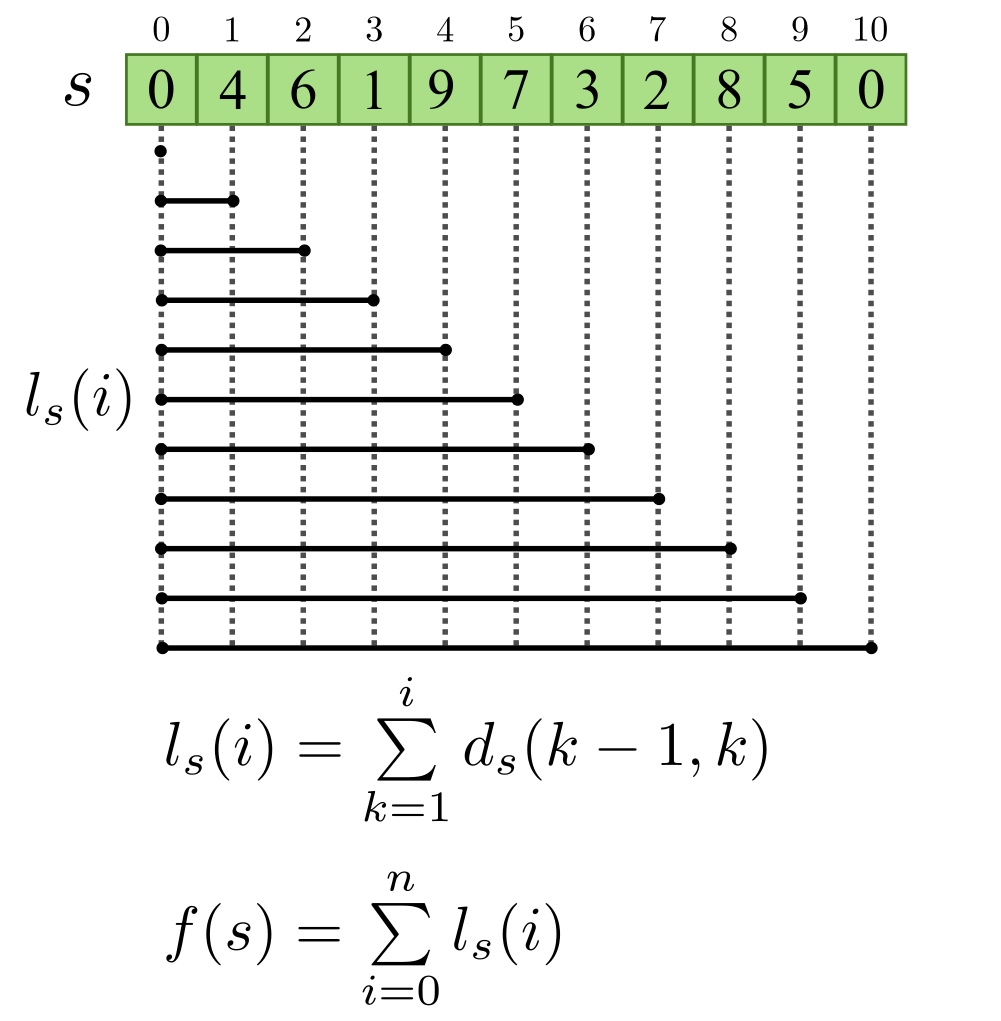
\includegraphics[width=0.6\linewidth]{figuras/pml/mlp}
    \caption{Exemplo de solução com as latências de cada cidade e cálculo da função objetivo}
    \label{fig:pmlDiagramaFormulas}
\end{figure}

O objetivo do PML é, iniciando do depósito, determinar o ciclo Hamiltoniano $s$ que minimize a latência expressa por $L(s)=\sum_{i=0}^{n} l(i)$ como pode ser visto na Figura~\ref{fig:pmlDiagramaFormulas}.
Assim sendo, uma solução viável do PML consiste numa permutação de $n$ clientes determinando a ordem de visita dos mesmos. Tomemos o exemplo a seguir, se $n=9$,  $s=[0,8,3,7,1,4,2,5,6,0]$ é uma solução viável para o PML (de fato, qualquer permutação $1..8$ começando e terminando no vértice zero é uma solução viável).

Apesar da formulação simples e de sua grande aplicação na otimização de latência em redes, o PML é um problema complexo, sendo provado que o PML é NP-Difícil~\cite{silva2012}. A despeito da semelhança na formulação do PML com a do Problema do Caixeiro Viajente (PCV) a sua função objetivo é mais complexa de ser calculada que a do PCV.
No PML, pequenas alterações no vetor solução podem levar a grandes alterações no resultado final da solução e a natureza não local da função objetivo faz com que uma simples inserção afete todas as latências subsequentes.
Na literatura, o PML também é conhecido Problema do Caixeiro Viajante Cumulativo \cite{bianco1993}, Problema do Entregador \cite{mladenovic2013} e Problema do Reparador Viajante. \cite{tsitsiklis1992}.

Em trabalhos recentes, um procedimento de busca local baseado em \emph{Graphics Processing Unit} (\emph{GPU}) e computação \emph{multi-core} foi proposto para o PML~\cite{wamca2016}.
A ideia foi chamada \emph{Distributed Variable Neighborhood Descent} (\emph{DVND}), tentando explorar diferentes estratégias de vizinhança simultaneamente para uma solução de entrada.

Em otimização, uma vizinhança é definida como um conjunto de operações chamados "movimentos", que são capazes de realizar pequenas alterações na solução de entrada.
Estas alterações podem ser, por exemplo, trocar dois elemento na permutação inicial, gerando dessa forma $\mathcal{O}(N^2)$ diferentes soluções (para o caso de uma permutação de tamanho $N$). Existe na literatura muitas dessas vizinhanças (como 2-Opt, OrOpt-1, OrOpt-2, Swap, ..., etc), conquanto por limitações computacionais estes são sempre explorados de forma sequencial, chamados de \emph{Variable Neighborhood Descent} (\emph{VND}).
Com o objetivo de encontrar um ótimo local para o PML, a ideia principal do DVND é usar GPU para obter operações de grão fino (que em geral são rápidas) e explorar toda a vizinhança $\mathcal{O}(N^2)$ mais rápido que em CPU (como explicado em~\cite{wamca2016}) e combinar as respostas das buscas, escolhendo a nova melhor solução.

\subsection{Exemplo}

% \begin{figure}[htpb]
%     \centering
%     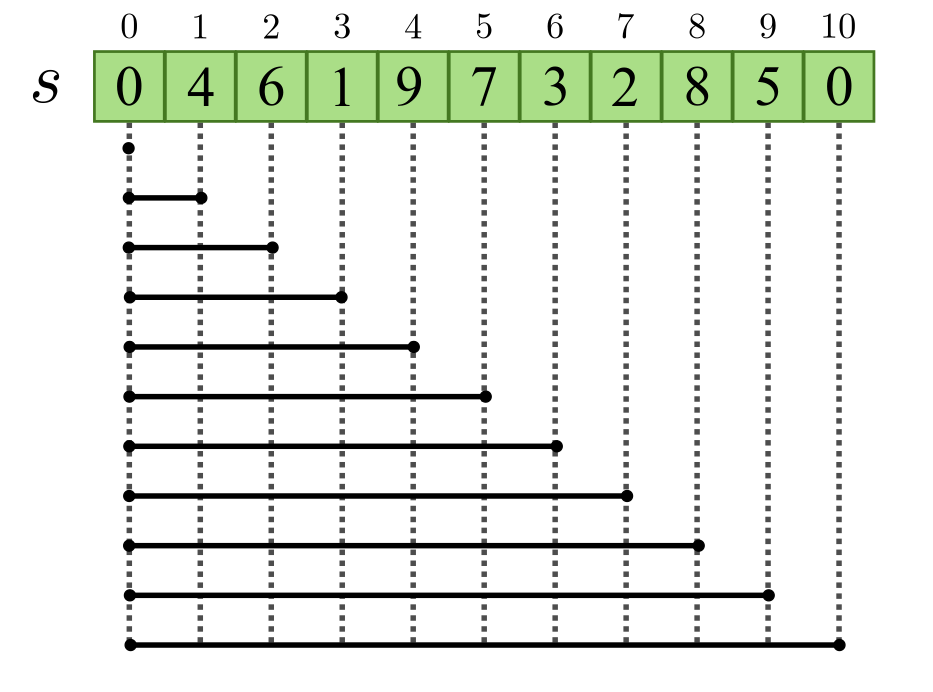
\includegraphics[width=0.6\linewidth]{figuras/pml/mlp-clean}
%     \caption{Exemplo de solução com as latências de cada cidade}
%     \label{fig:pml}
% \end{figure}

Pelo exemplo na Figura~\ref{fig:pmlDiagramaFormulas} podemos ver que o valor da latência $L(s)$ será dado palos somatórios das latências de todas as cidades, sendo $d_s^{i, j}$ a distância da cidade $i$ para a cidade $j$ na solução $s$, então temos:
$$ L(s) = \sum_{i=0}^n{l_s(i)} $$
$$ L(s) = l_s(0) + l_s(1) + l_s(2) + l_s(3) + l_s(4) + l_s(5) + l_s(6) + l_s(7) + l_s(8) + l_s(9) $$
$$ L(s) = 10d_s^{0, 4} + 9d_s^{4, 6} + 8d_s^{6, 1} + 7d_s^{1, 9} + 6d_s^{9, 7} + 5d_s^{7, 3} + 4d_s^{3, 2} + 3d_s^{2, 8} + 2d_s^{8, 5} + d_s^{5, 0}$$
